\subsection{Election November 8, 1864: *Lincoln vs McClellan}
\begin{frame}[t]{Election November 8, 1864: *Abraham Lincoln}
\small
% Lincoln
\begin{columns}[T, onlytextwidth]
\column{0.48\textwidth}
\vspace{-1em}
{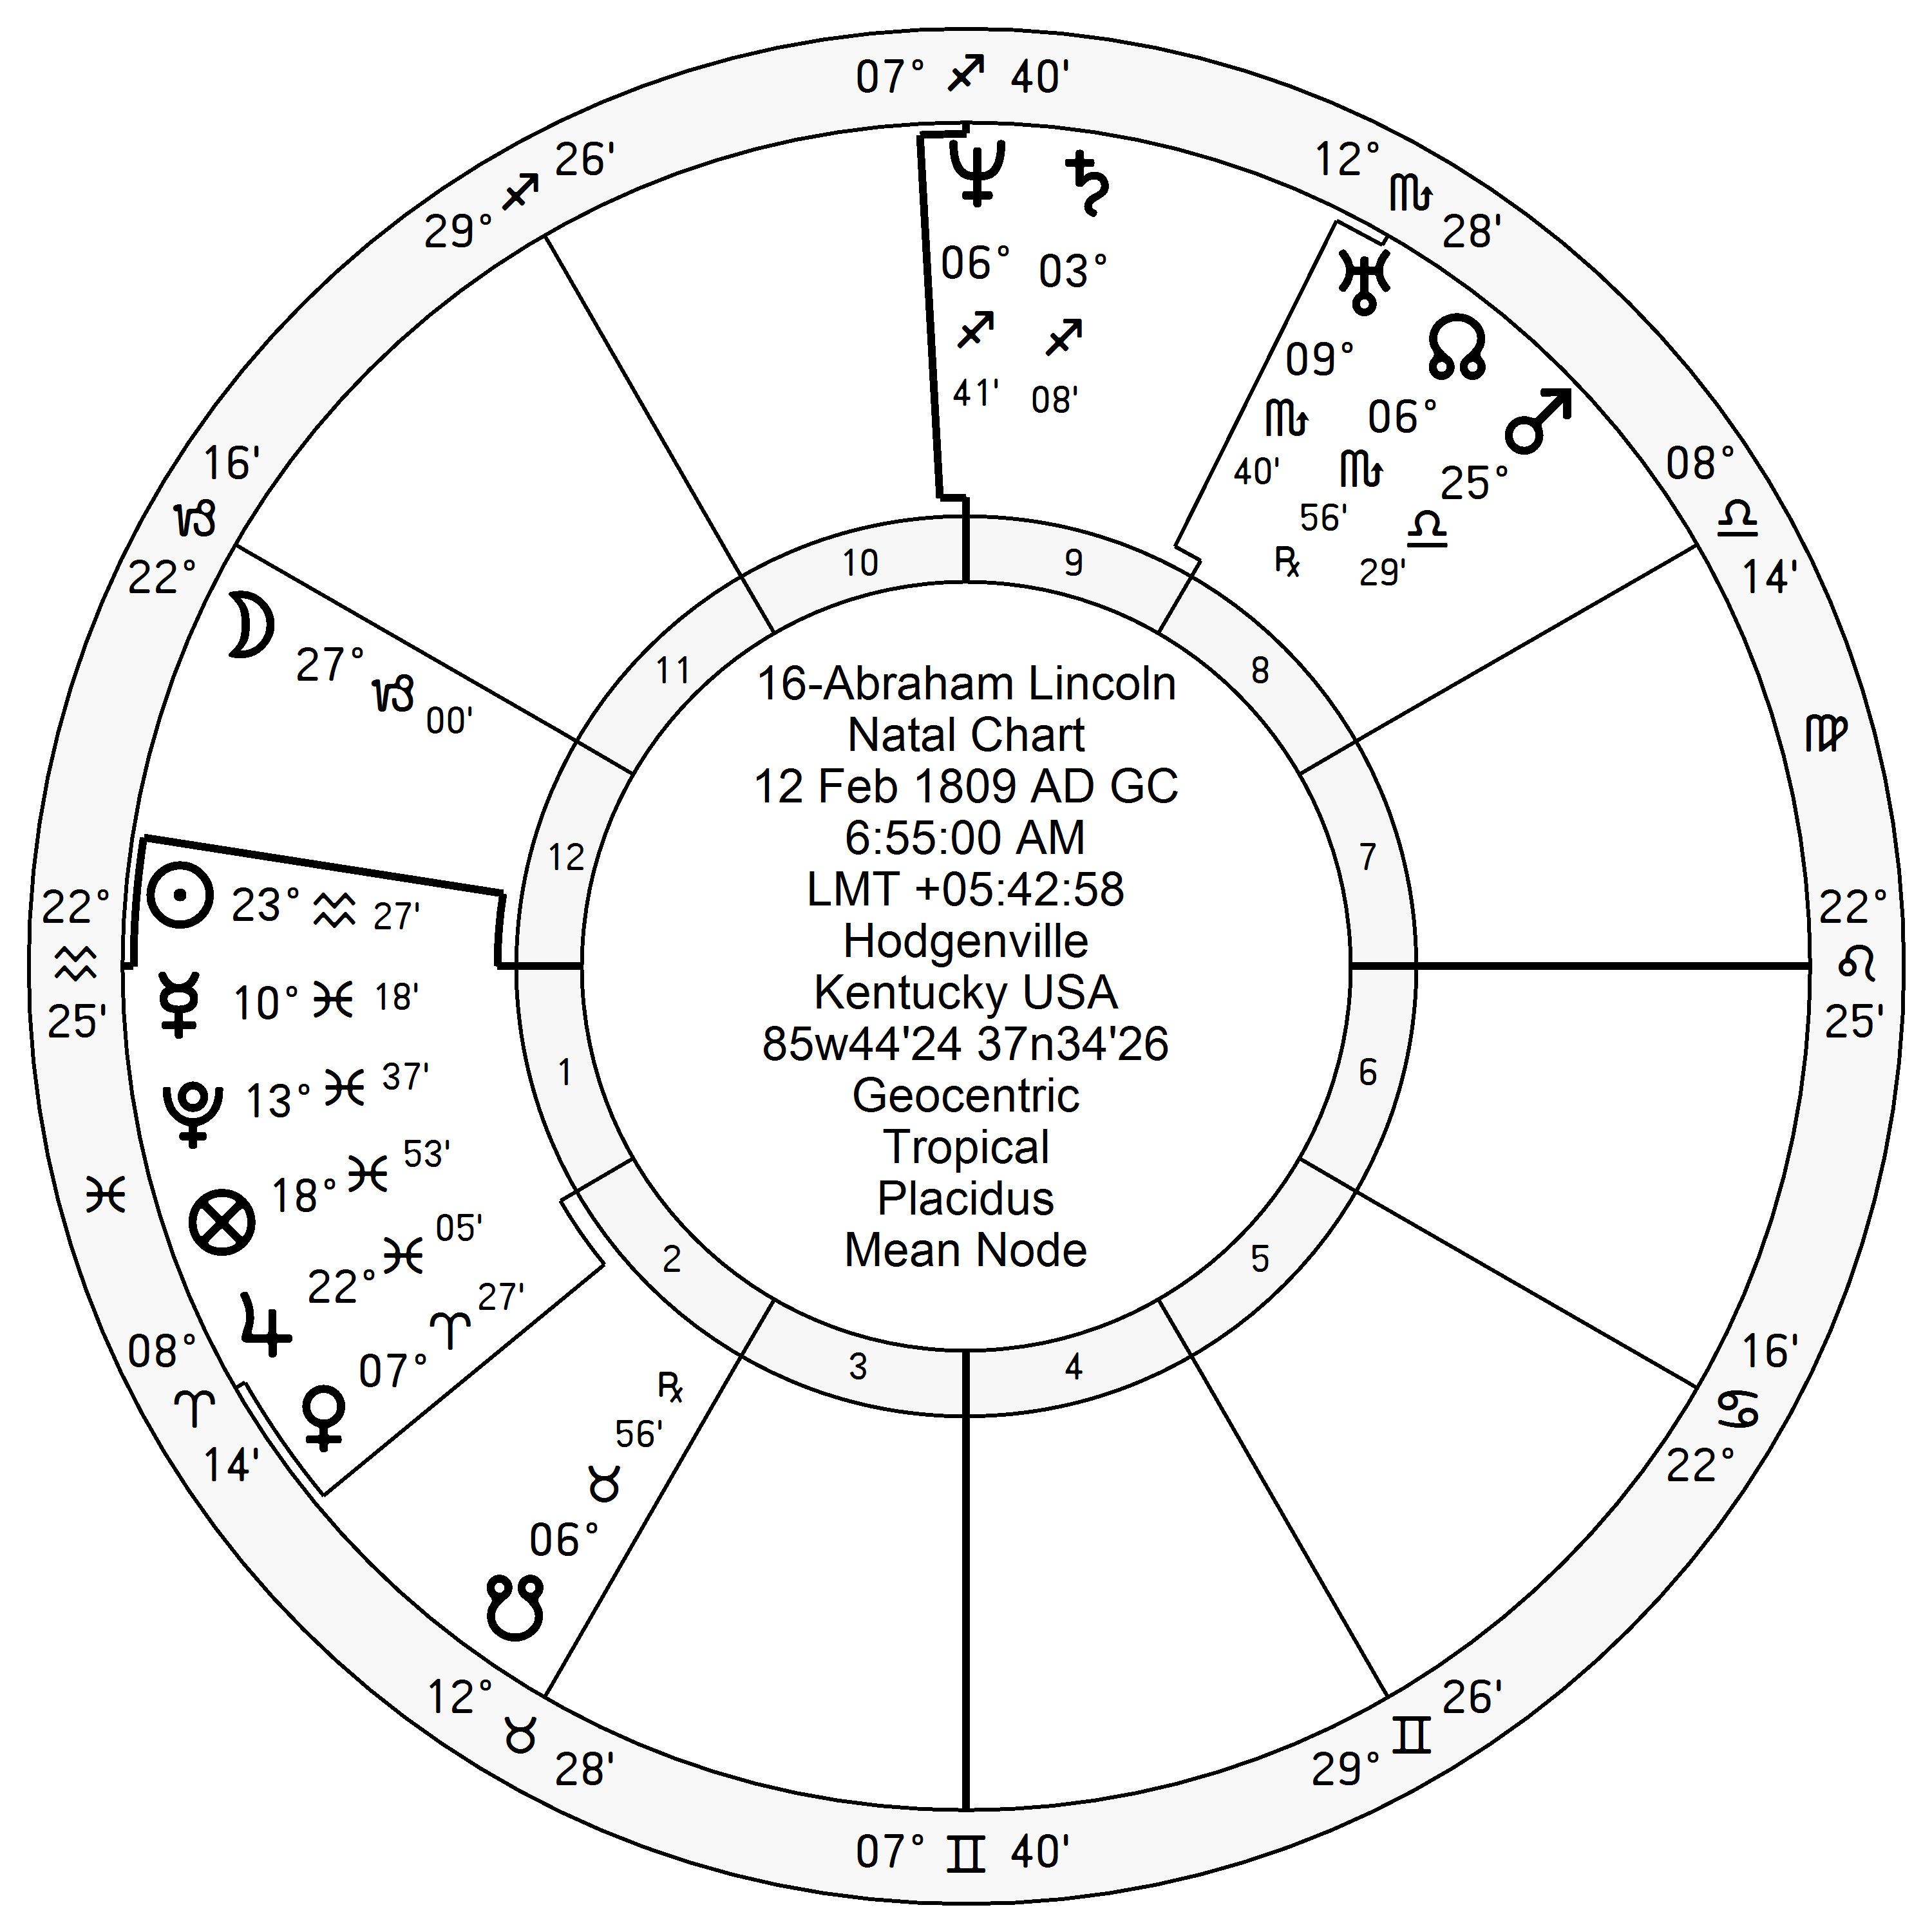
\includegraphics[width=0.9\textwidth]{charts/Lincoln.png}}
\fontsize{7pt}{8pt}\selectfont

\Mercury\, \Trine\, P10, \textbf{\Square\, N10} \\
\Venus\, \textbf{\Square\, P10}; in N1 partile \Trine\, MC

\column{0.48\textwidth}
\vspace{-1em}
{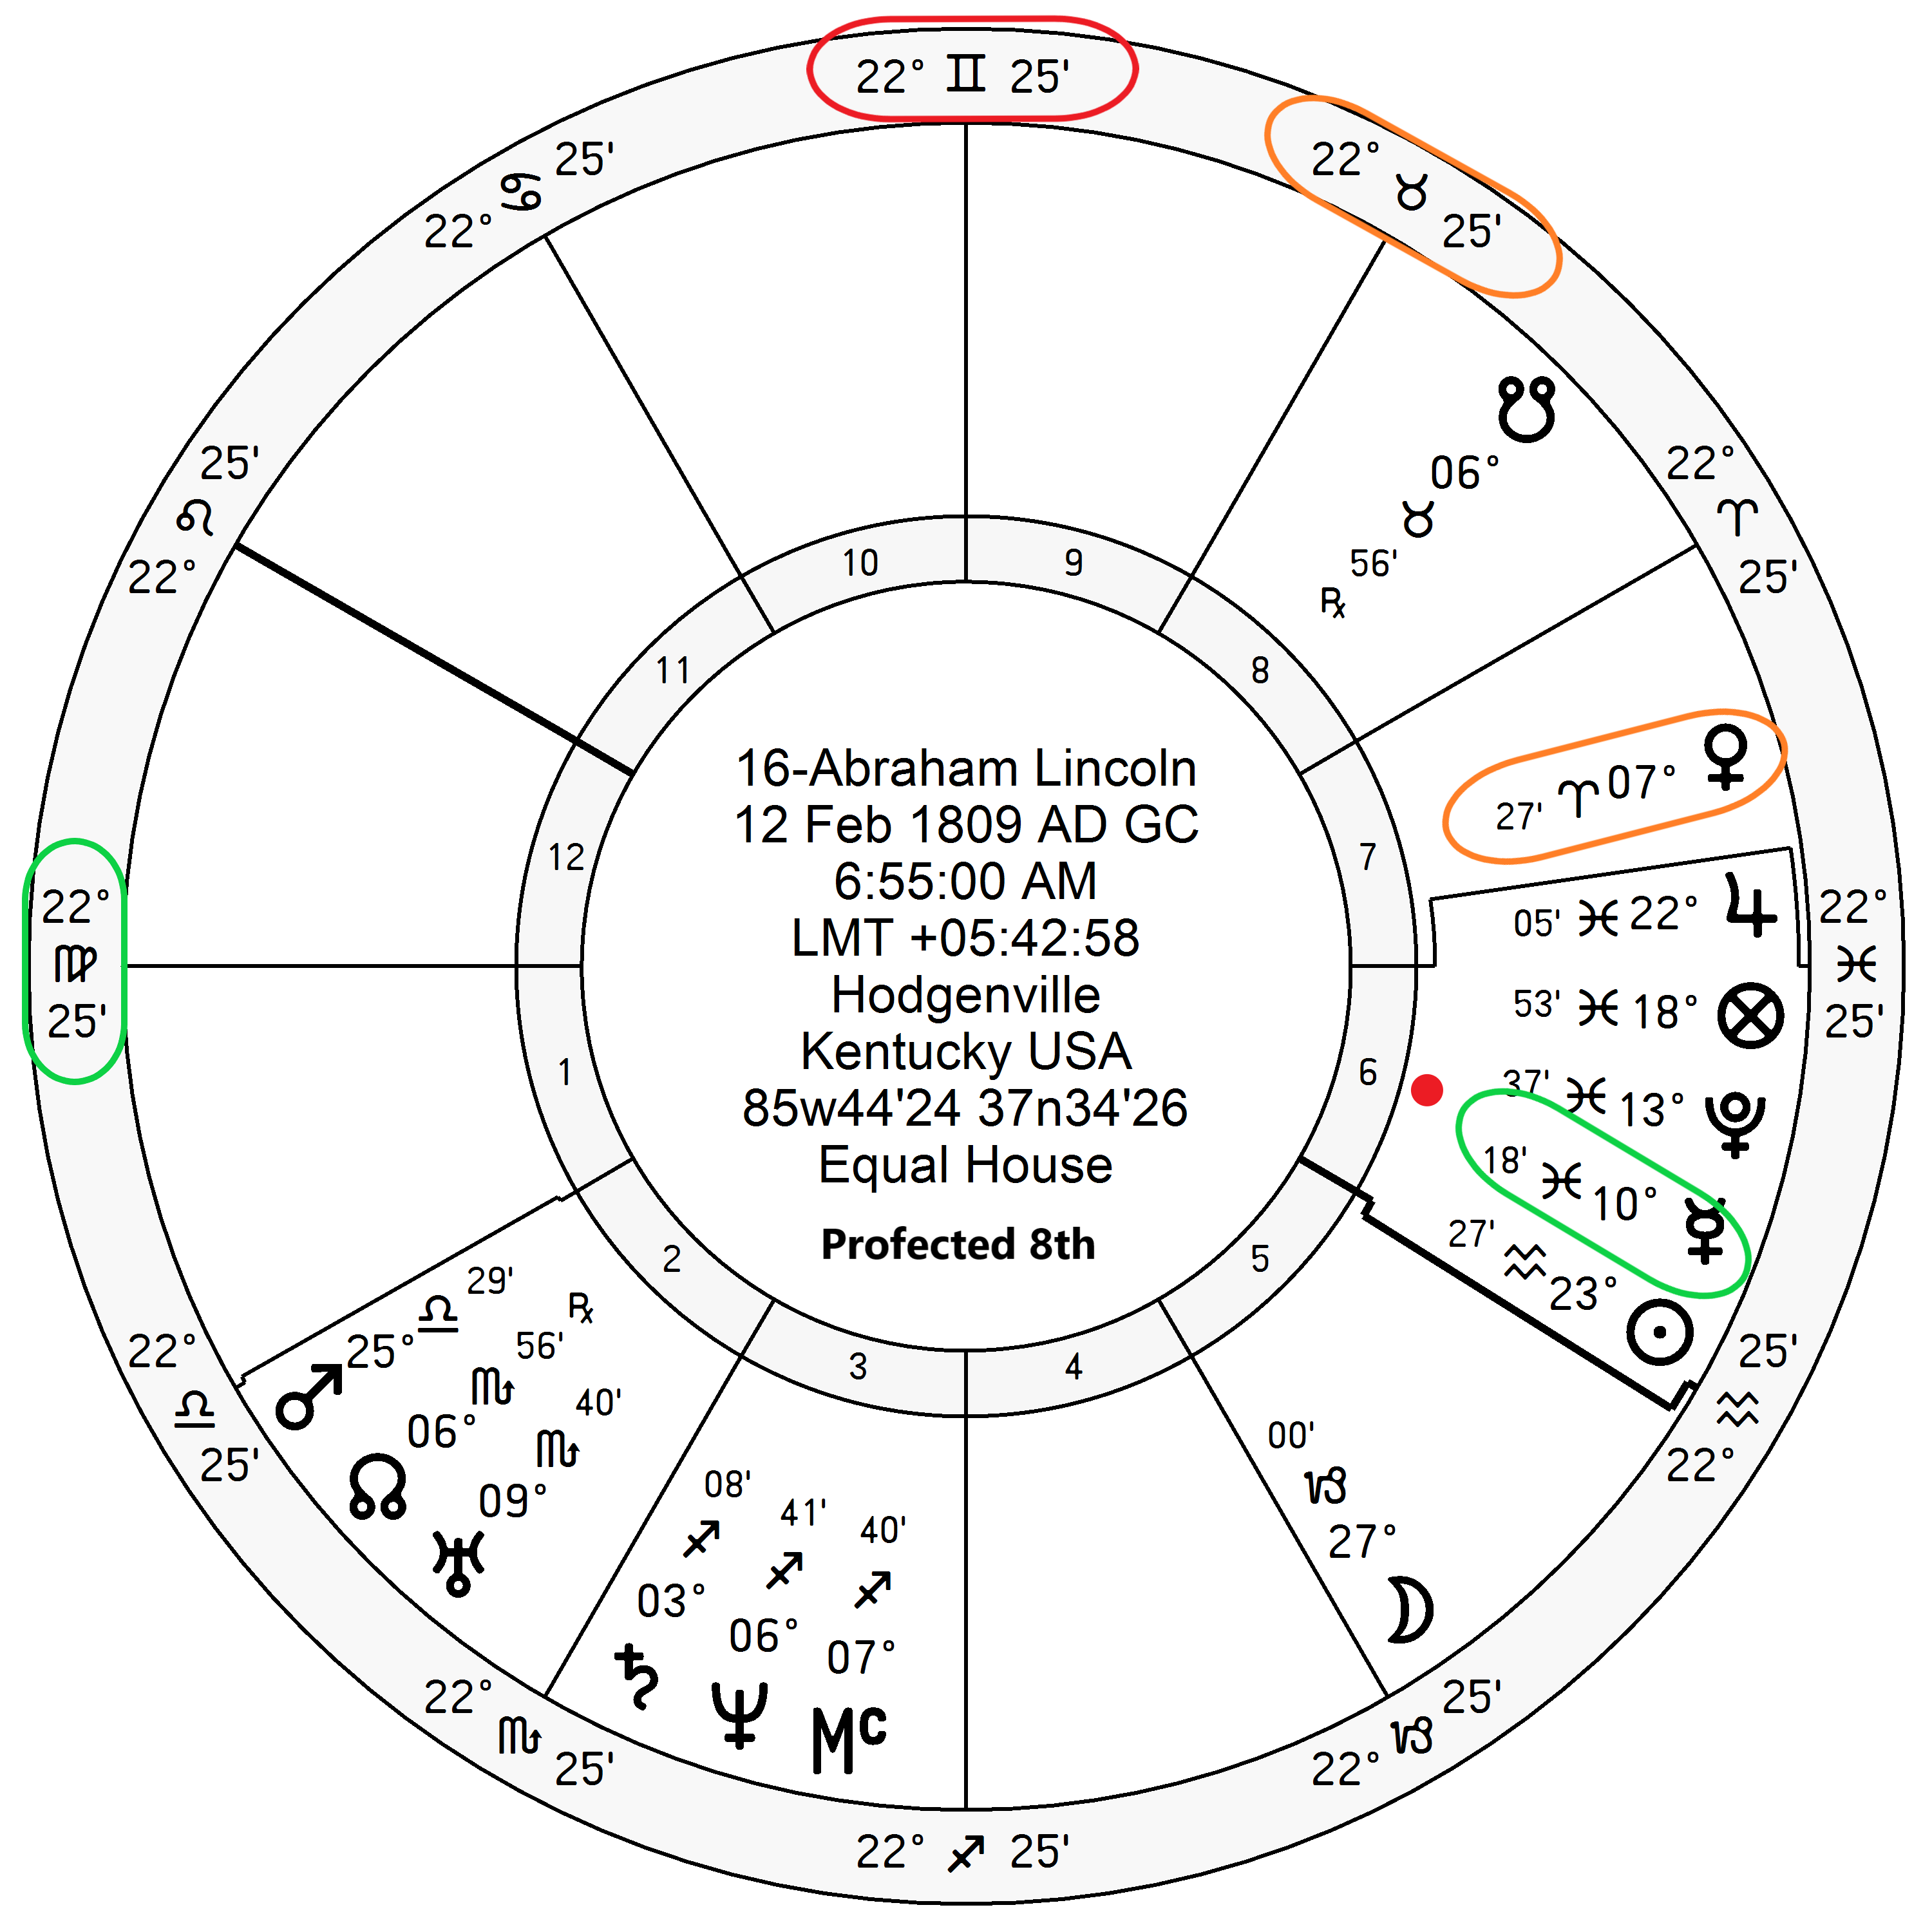
\includegraphics[width=0.9\textwidth]{charts/Lincoln-Prof-8th.png}}
\textbf{\dgreen P1=N7} $\Rightarrow$ \Mercury\, $\Rightarrow$ \textbf{\dgreen P6/N1} \\
\textbf{\red{P10}}=N4 $\Rightarrow$  \Mercury\, $\Rightarrow$  \textbf{\dgreen{P6/N1}} \\
PE=P9/N3 $\Rightarrow$  \Venus\, $\Rightarrow$  \textbf{\dgreen{P7/N1}}

\end{columns}
\end{frame}

% McClellan
\begin{frame}[t]{Election November 8, 1864: George McClellan}
\small
\begin{columns}[T, onlytextwidth]
\column{0.48\textwidth}
\vspace{-1em}
{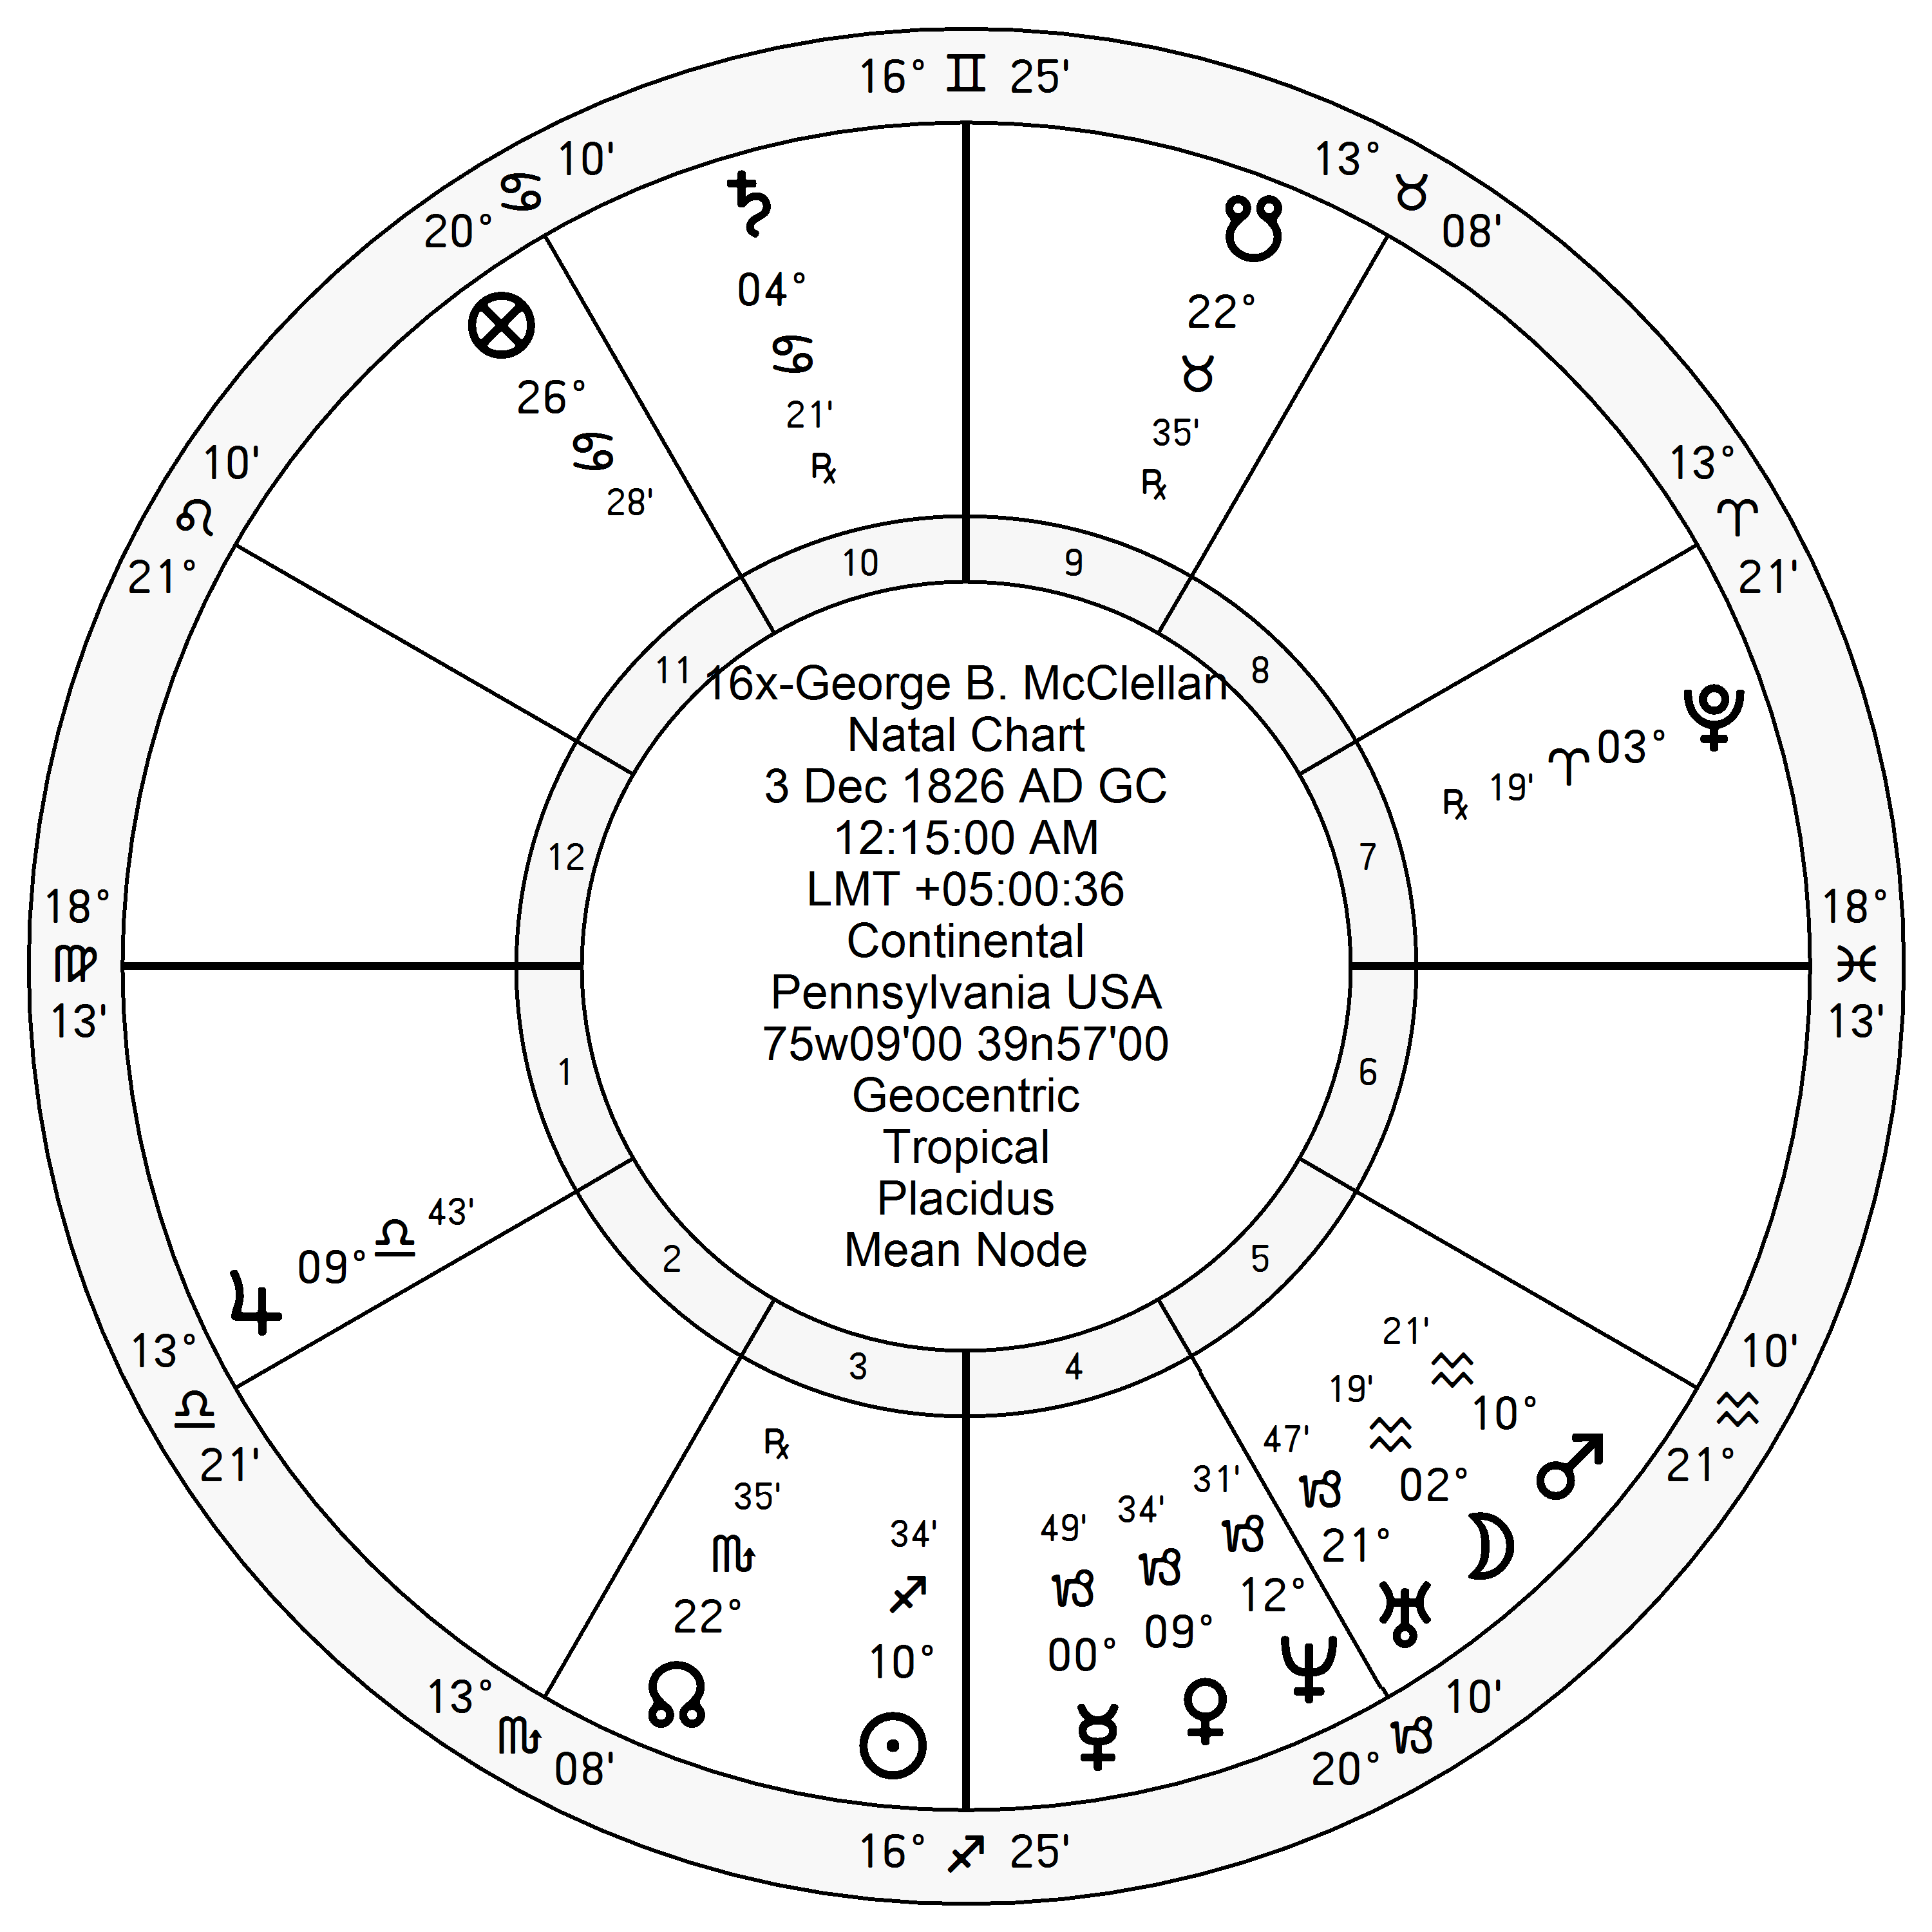
\includegraphics[width=0.9\textwidth]{charts/McClellan.png}}
\fontsize{8pt}{9pt}\selectfont

\Venus\, \Sextile\, P1, N1 \\
\Moon\, \textbf{\Opposition\, P10} \\
\Mercury\, \Sextile\, P1, N1 \\


\column{0.48\textwidth}
\vspace{-1em}
{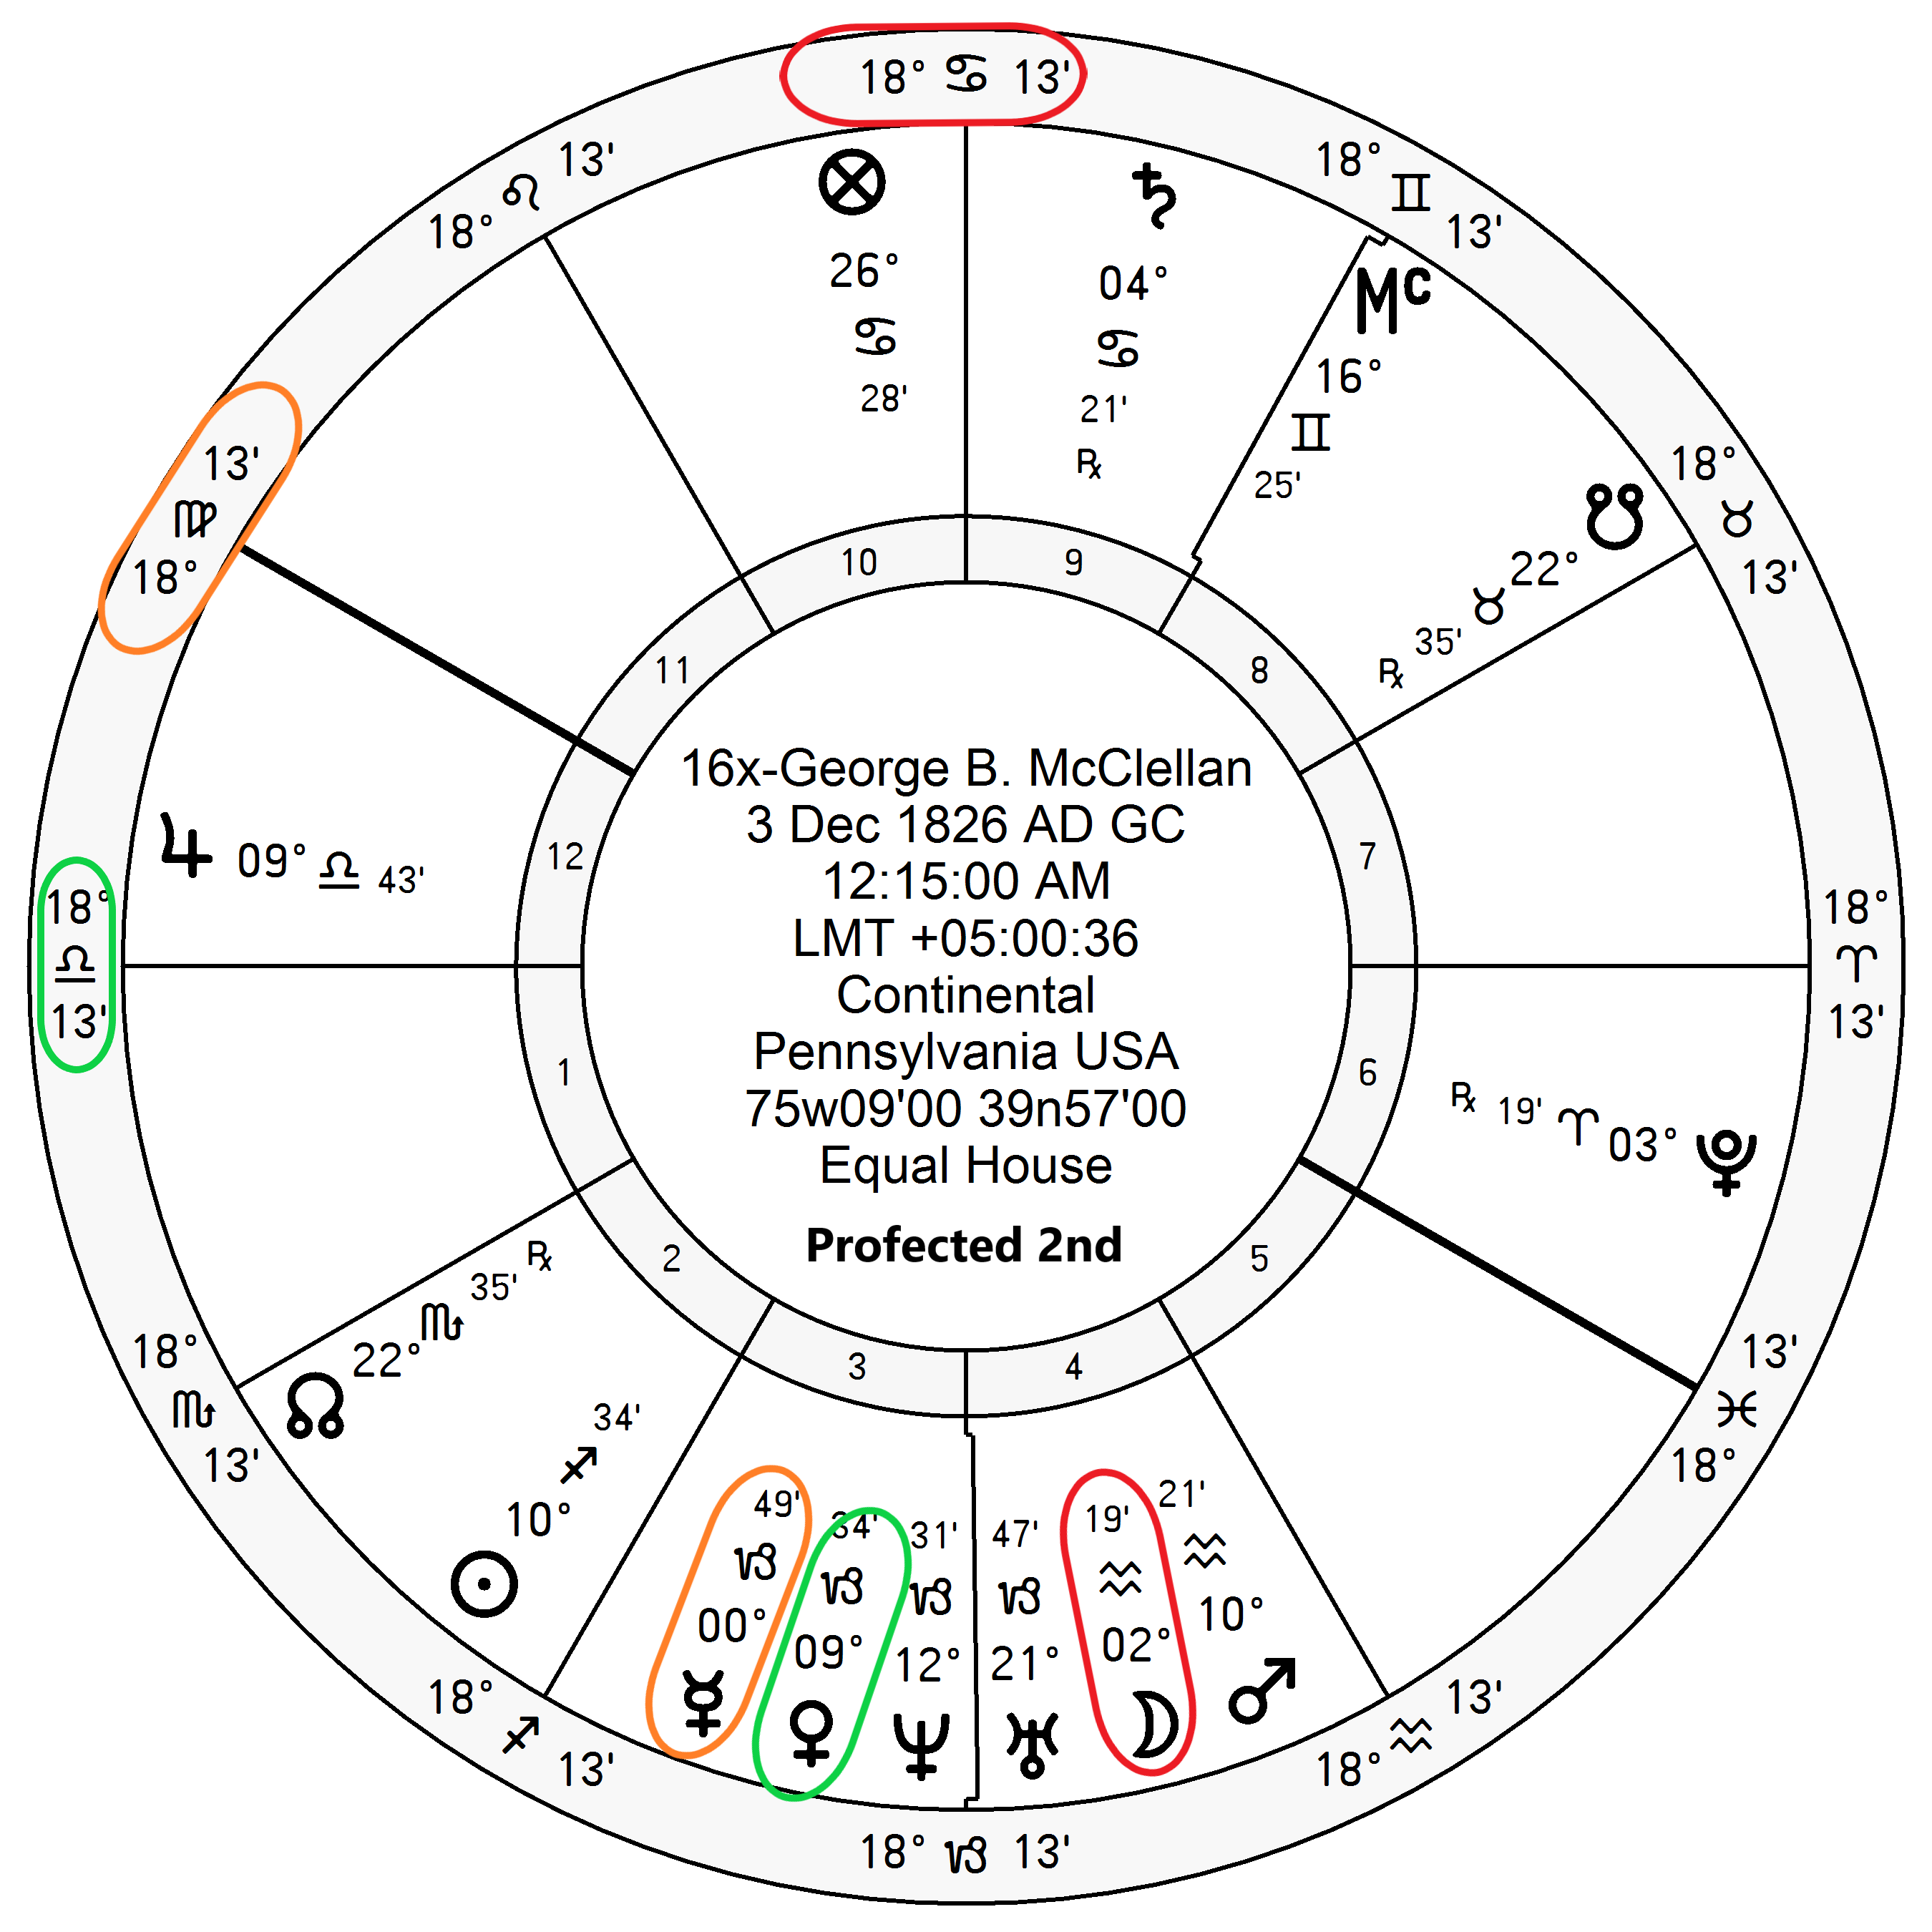
\includegraphics[width=0.9\textwidth]{charts/McClellan-Prof-2nd.png}}
\textbf{\dgreen P1}=N2 $\Rightarrow$ \Venus\, $\Rightarrow$ \textbf{\dgreen P3/N4}\\
\textbf{\red P10}=N11 $\Rightarrow$ \Moon\, $\Rightarrow$ \textbf{\dgreen P4}/N5\\
PE=P12/\textbf{\dgreen N1} $\Rightarrow$ \Mercury\, $\Rightarrow$ \textbf{\dgreen P3/N4}

\end{columns}
\end{frame}
